\section{Mô phỏng thuật toán giải mã Viterbi bằng C}

\begin{figure}[H]
	\centering
	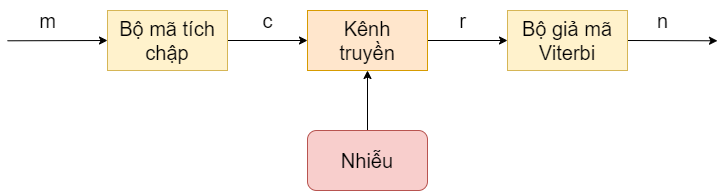
\includegraphics[width=.8\linewidth]{sections/pic/mophongbangC/system_conv.png}
	\caption{Sơ đồ khối hệ thống.}
	\label{f_system_conv}
\end{figure}

Tín hiệu sau khi được số hóa thành các bit, các bit này sẽ được đưa đến bộ mã hóa Mã chập. Sau khi được mã hóa, tín hiệu (các bit) đươc truyền qua kênh truyền có nhiễu, ở đây có thể coi nhiễu là nhiễu Gauss trắng. Tín hiệu đã bị thay đổi bởi nhiễu được thu vào và giải mã bởi bộ giải mã Viterbi. Ngờ thuật toán Viterbi, tín hiệu được giải mã sẽ gần giống nhất với tín hiệu ban đầu.

Dựa vào hình \ref{f_system_conv}, ta thực hiện theo sơ đồ sau:

\begin{figure}[H]
	\centering
	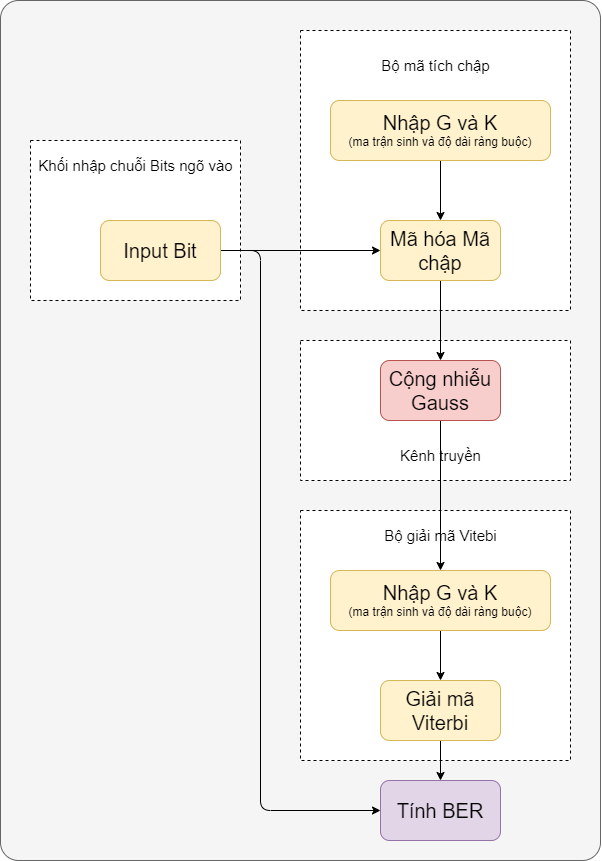
\includegraphics[width=.6\linewidth]{sections/pic/mophongbangC/flowchart_diagram_withC.png}
	\caption{Lưu đồ mô phỏng.}
\end{figure}

\subsection{Khối nhận chuỗi Bits đầu vào}

Cho phép người dùng nhập giá trị chuỗi bit đầu vào ở dạng chuỗi (\texttt{char}) và chuỗi chuỗi vừa nhận thành mảng một chuỗi chứa các giá trị số thực (\texttt{int}).

% Thêm đoạn code hiển thị kết quả ở đây

\subsection{Bộ mã tích chập}

Với việc mô phỏng bộ Viterbi ($3, 1, 2$), thì giá trị $G$ và $K$ được cho trước là:

\[
	G = \begin{bmatrix}
		1 & 1 & 1\\
		1 & 0 & 1
	\end{bmatrix}, K = 3
\]

Ta có lưu đồ giải thuật của Bộ mã Tích chập,

\begin{figure}[H]
	\centering
	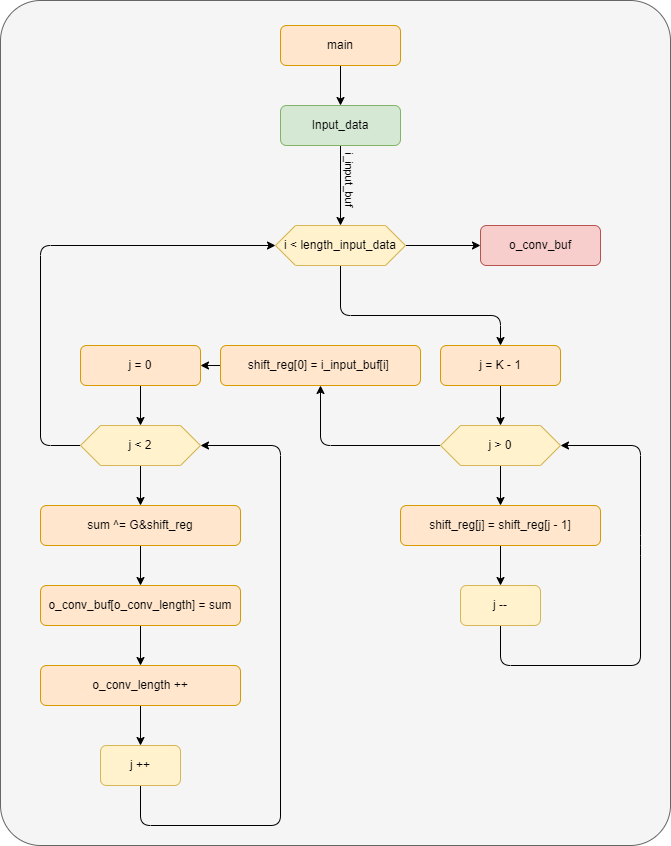
\includegraphics[width=.8\linewidth]{sections/pic/mophongbangC/flowchart_conv_block_withC.png}
	\caption{Lưu đồ giải thuật của Bộ mã Tích chập.}
\end{figure}

\subsection{Bộ giải mã Viterbi}

\begin{figure}[H]
	\centering
	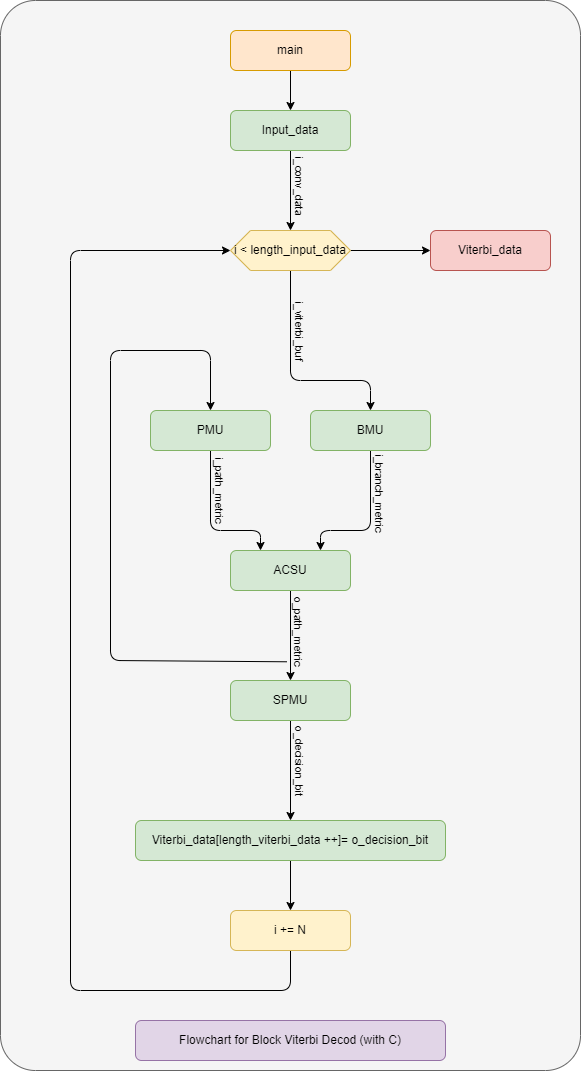
\includegraphics[width=.6\linewidth]{sections/pic/mophongbangC/flowchart_VD_312.png}
	\caption{Lưu đồ giải thuật của Bộ giải mã Viterbi.}
\end{figure}

\subsection{Kết quả}

\begin{lstlisting}[style=StyleResult]
	------------------- Input Data -------------------
	Input data: 110110
	The constraint length K = 3
	The number of input M = 1
	The number of output N = 2
	Enter the Generator Polynomial Matrix (G[n][k]): = [(1 1 1) (1 0 1)]
	
	Input data: 110110
	
	------------- Ouput Conv Data -------------
	
	Conv Data: 110101000101
	
	
	------------------- Input Data -------------------
	Input data: 110110
	The constraint length K = 3
	The number of input M = 1
	The number of output N = 2
	Enter the Generator Polynomial Matrix (G[n][k]): = [(1 1 1) (1 0 1)]
	
	Input data: 110110
	
	------------- Ouput Conv Data -------------
	
	Conv Data: 110101000101
	
	------------- Viterbi Decoder -------------
	Viterbi data: 110101000101
	
	Input Viterbi: 11
	BM0 = 2, BM1 = 1, BM2 = 1, BM3 = 0
	iPM0 = 0, iPM1 = 3, iPM2 = 3, iPM3 = 3
	oPM0 = 2, oPM1 = 4, oPM2 = 0, oPM3 = 4
	State = 1
	Nex State = 3
	Decision Bit = 1
	Input Viterbi: 10
	BM0 = 1, BM1 = 0, BM2 = 2, BM3 = 1
	iPM0 = 2, iPM1 = 4, iPM2 = 0, iPM3 = 4
	oPM0 = 3, oPM1 = 2, oPM2 = 3, oPM3 = 0
	State = 3
	Nex State = 4
	Decision Bit = 1
	Input Viterbi: 10
	BM0 = 1, BM1 = 0, BM2 = 2, BM3 = 1
	iPM0 = 3, iPM1 = 2, iPM2 = 3, iPM3 = 0
	oPM0 = 3, oPM1 = 0, oPM2 = 3, oPM3 = 2
	State = 4
	Nex State = 2
	Decision Bit = 0
	Input Viterbi: 00
	BM0 = 0, BM1 = 1, BM2 = 1, BM3 = 2
	iPM0 = 3, iPM1 = 0, iPM2 = 3, iPM3 = 2
	oPM0 = 2, oPM1 = 3, oPM2 = 0, oPM3 = 3
	State = 2
	Nex State = 3
	Decision Bit = 1
	Input Viterbi: 10
	BM0 = 1, BM1 = 0, BM2 = 2, BM3 = 1
	iPM0 = 2, iPM1 = 3, iPM2 = 0, iPM3 = 3
	oPM0 = 3, oPM1 = 2, oPM2 = 3, oPM3 = 0
	State = 3
	Nex State = 4
	Decision Bit = 1
	Input Viterbi: 10
	BM0 = 1, BM1 = 0, BM2 = 2, BM3 = 1
	iPM0 = 3, iPM1 = 2, iPM2 = 3, iPM3 = 0
	oPM0 = 3, oPM1 = 0, oPM2 = 3, oPM3 = 2
	State = 4
	Nex State = 2
	Decision Bit = 0
	Viterbi Data: 110110
\end{lstlisting}

%\lstinputlisting[style=StyleCode, language=C, caption={SystemVerilog Example}]{../01_system_lever_test/VD_312/VD_312.c}